\documentclass[11pt,journal]{IEEEtran}
\usepackage{lipsum}
\usepackage[T1]{fontenc}
\usepackage{fouriernc}
\usepackage{cases}
\usepackage{amsmath}
\usepackage[noadjust]{cite}
\usepackage{hyperref}
\usepackage{multirow}
\usepackage{graphicx}
\usepackage{adjustbox}
\usepackage{makecell}
\usepackage[dvipsnames]{xcolor}
\usepackage{tikz}
\usepackage{lipsum}
\usepackage{listings}

\hypersetup{
    colorlinks=true,
    linkcolor=blue,
    anchorcolor=blue,
    urlcolor=blue,
    citecolor=blue
}

\newcommand{\eq}{\; = \;}
\newcommand{\text}[1]{\mbox{\footnotesize #1}}
\newcommand{\nl}{

\medskip

}
\newcommand{\centered}[2]{\begin{tabular}{#1} #2 \end{tabular}}

\lstdefinestyle{standstyle}{
    %backgroundcolor=\color{backcolour!05},
    basicstyle=\ttfamily\linespread{1}\scriptsize\color{black!80},
    breakatwhitespace=false,
    breaklines=true,
    captionpos=b,
    keepspaces=true,
    numbers=none,
    numbersep=5pt,
    showspaces=false,
    showstringspaces=false,
    showtabs=false,
    tabsize=4,
}

\lstset{style=standstyle}

\title{GuNiLeo: Lip Reading From Videos With STCNN}
\author{Beray Nil Atabey (\textit{2045576}) \quad Leonardo Biason (\textit{2045751}) \quad Günak Yüzak (\textit{2048950})}

\begin{document}

\maketitle

\begin{abstract}
    Lip reading is a task that can have various usages as an accessibility feature, but it's also very complex to design: it requires a machine to be able to differentiate between the various words said by a speaker, and also to predict what the speaker said whenever words aren't spelled with a precise motion of the lips. With this paper, we propose a model based on a Spatio-Temporal CNN, capable of reading the words said by a speaker from a video clip of maximum 75 frames.
\end{abstract}

\section{Introduction}

\lipsum[1]

\section{Implementation}

In order to create a lip reading model, the following steps have been undertaken:
\begin{itemize}
    \item [1)] creation and modeling of the dataset;
    \item [2)] creation of the model;
    \item [3)] training of the model;
    \item [4)] evaluation of the model.
\end{itemize}

\section{Creation and Modeling of the Dataset}

The project adopted an already existing dataset from the University of Sheffield: such dataset is called \textsc{Lombard Grid} \cite{gunileo:dataset}.

\subsection{Structure of the Dataset}

The dataset comprehends two fundamental parts: the data part and the labels. The data consists in a set of 5000+ videos, where each video records frontally a person saying a specific sentence. Each sentence is then transcribed in a \texttt{json} file, which has the following format:

\begin{itemize}
    \item \texttt{video\_name}: a list containing all the phonemes and the timing of said phonemes of a clip;
    \begin{itemize}
        \item \texttt{duration}: the duration in seconds of the phoneme;
        \item \texttt{offset}: the beginning of the phoneme, with respect to the beginning of the video;
        \item \texttt{phone}: an encoding of the phoneme.
    \end{itemize}
\end{itemize}

\begin{figure}
    \renewcommand{\arraystretch}{1.3}
    \caption{Example of frame (on the left) and label (on the right)}
    \label{frame_label}

    \begin{tabular}{c c}
        \centered{c}{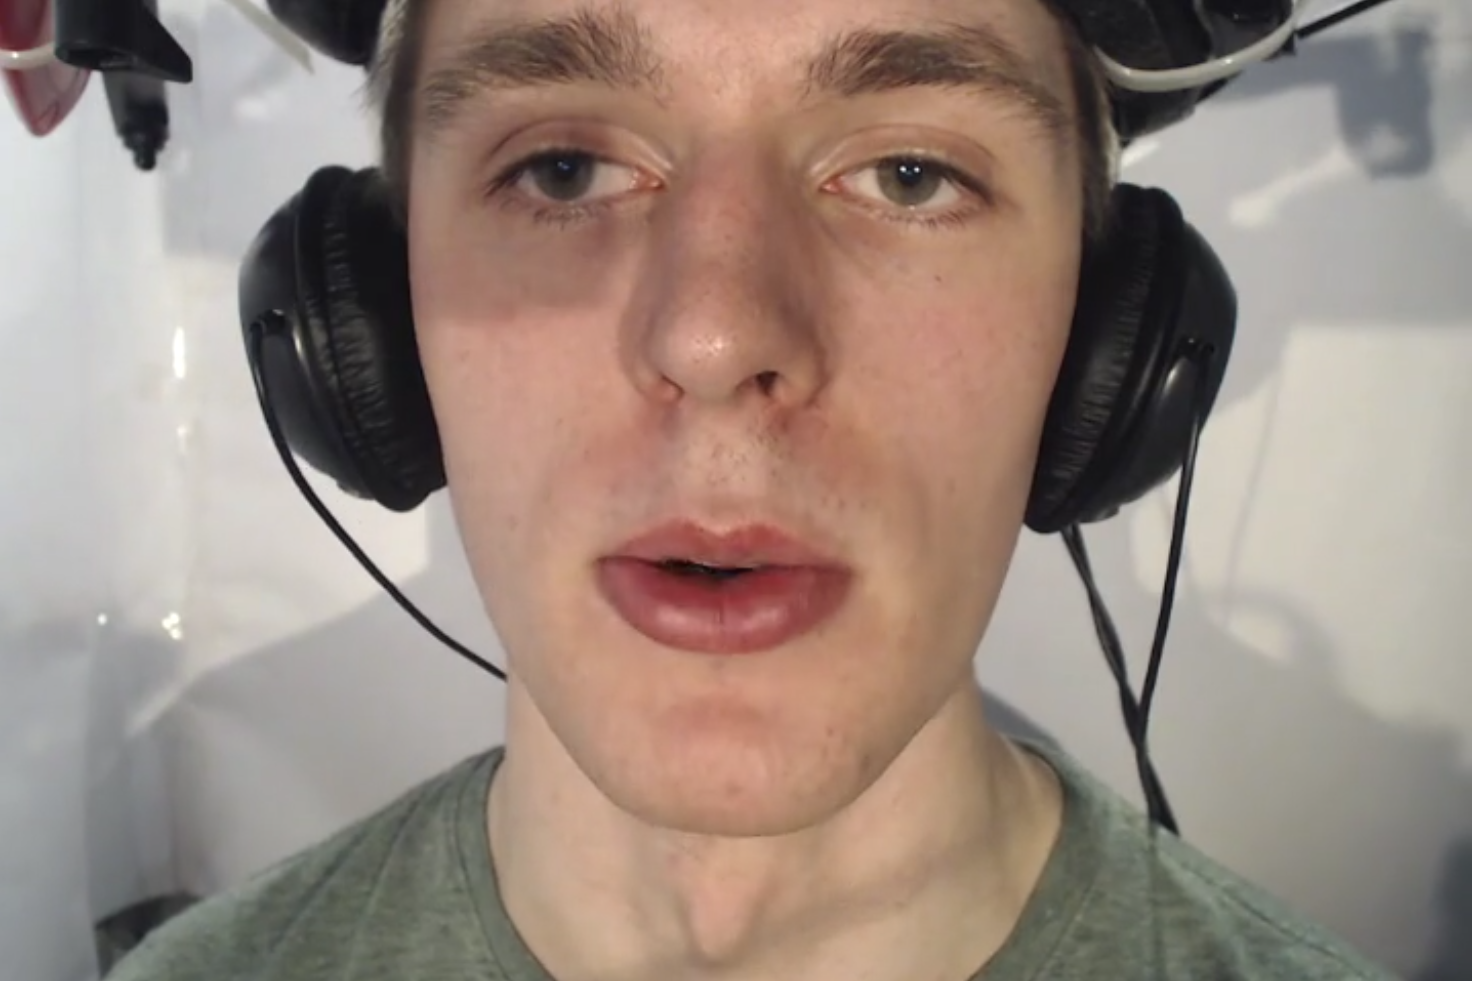
\includegraphics[width = 0.3\linewidth]{images/001_frame.PNG}} & \begin{lstlisting}[language = json]
{
    "video_name": [
        {
            "duration": 0.01,
            "offset": 0,
            "phone": "SIL_S"
        }
    ]
}
            \end{lstlisting} \\
        {\scriptsize Frame} & {\scriptsize Label} \\
    \end{tabular}
\end{figure}

\nl
An example of data-label pair can be observed in Figure \ref{frame_label}, where a frame of a sample video has been reported, alongside an example of possible label. The label can be interpreted as follows: there is a phoneme, the silent "s", which starts at $t \eq 0$ and lasts for $0,01s$.

\subsection{Pre-processing of the Dataset}

Since we want to read the lips, the only area that concerns us is the mouth and the close surroundings. The rest of the video can be cropped to avoid unnecessary memory-wise and computational power-wise waste. In order to locate the mouth, the \texttt{dlib} \cite{gunileo:dlib} library's face detection and landmark detection algorithm has been employed. The face detection is implemented in \texttt{dlib} itself, however for the landmark an external model had to be used. We now proceed to describe the undertaken steps for the pre-processing of the data:
\begin{itemize}
    \item [1)] First, the face detection algorithm is ran on the video in order to find the coordinates of the face;
    \item [2)] Such coordinates are given as input into the landmark model, which determines the important landmarks of the face via a sequence of 68 points. Points from 49 to 68 determine where the mouth is (such points are shown in Figure \ref{face_landmark_points});
    \item [3)] From these points, it's possible to find the points that are on the left,right, up and down most of the mouth, which correspond to the maximum coordinates that a mouth can take in a specific video;
    \item [4)] From these coordinates a margin distance is added, and after that the video gets cropped around the mouth. Clearly, every person's mouth size is different from one another, so the resize procedure reshapes the video to a fixed size of $150 \times 100$ pixels;
    \item [5)] Finally, the resized video is then grayscaled and normalized for a better performance of the model.
\end{itemize}

\begin{figure}
    \centering{
        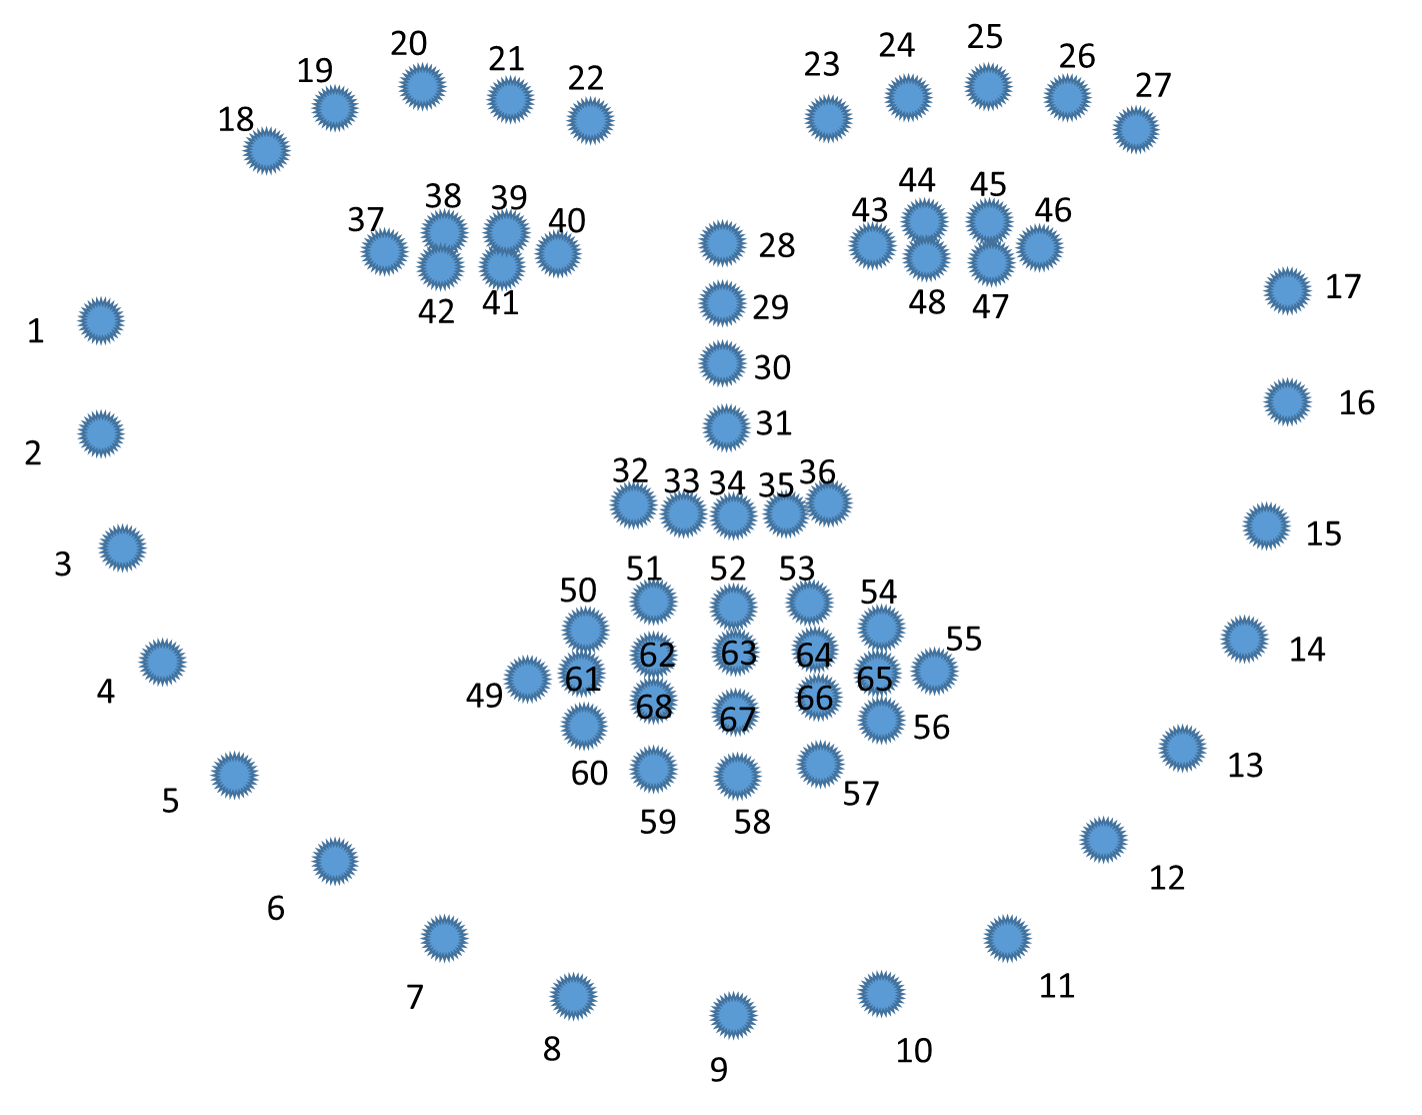
\includegraphics[width = 0.7\linewidth]{images/002_face_landmark_representation.png}
    }
    \renewcommand{\arraystretch}{1.3}
    \caption{Face landmarking points}
    \label{face_landmark_points}
\end{figure}

\section{Architecture of the Model}

The model used for this project takes large advantage of the \textsc{Spatio-Temporal Convolutional Neural Network} concept \cite{gunileo:stcnn} (from now on referred to as STCNN). The choice of using such type of neural network is because of its capabilities of retaining information in the long short-term, which is very helpful when it comes to analysing multiple videos and making predictions on the long run.
\nl
Here follows the detailed architecture of our model, with all its layers:
\begin{itemize}
    \item STCNN and 3D Max Pooling $\times 3$:
    \item Bi-directional GRU unit $\times 2$:
    \item CTC loss function:
    \item Softmax activation function:
\end{itemize}

As input, the model takes a clip of size $(100, \; 150, \; 75, \; 1)$, and it returns a tensor of shape $(75, \; 37)$. The possible output, once encoded, is a list composed by letters from a-z, numbers from 0-9 or blank spaces "\textvisiblespace".
%HERE YOU CAN PUT THE SUMMARY IMAGE OF THE MODEL
\nl
The model supports 75 frames videos, which is a video of 3 seconds with a constant frame rate of 25$f$. The videos that had more than 75 frames are discarded from the dataset, and less then 75 frames are extended with 0 matrices.

\bibliographystyle{IEEEtran}
\bibliography{IEEEabrv, bibliography}

\end{document}
